\section{Iterator-Muster}

\subsection{Problemstellung}
Beispiel aus dem Buch: Zwei verschiedene Speisekarten sollen beide von einer Kellner-Klasse verwendet werden. Die Kellnerin soll in der Lage sein, alle Gerichte gemeinsam auszugeben, sowie die einzelne Gerichte zu filtern (Fr"uhst"uckstisch, etc.). Problem hierbei, die vorgegebenen Klassen nutzen jeweils eine andere Listenimplementierung. Wie kann man nun dennoch geschlossen "uber die Listen iterieren ohne den kompletten vorgegebenen Code umzuschreiben. 

\subsection{Erkl"arung des Musters}
\emph{Das Iterator-Muster bietet eine M"oglichkeit, auf die Elemente in einem Aggregat-Objekt sequenziell zuzugreifen, ohne die zu Grunde liegende Implementierung zu offenbaren.}
Das Muster gibt die Aufgaben der Durchquerung au"serdem dem Iterator-Objekt statt dem Aggregat. Das vereinfacht die Schnittstelle und die Implementierung des Aggregats und schiebt die Verantwortung f"ur die Iteration dahin, wo sie hingeh"ort. 

Um das beschriebene Problem zu l"osen reicht es die Iterator-Schnittstelle zu implementieren. Diese kapselt die Iteration und die Kellnerin kann nun polymorph "uber alle Elemente iterieren. Eine "ubergeordnete Speisekarten-Schnittstelle l"asst nun folgendes UML-Diagramm entstehen: 

\subsection{Punkt f"ur Punkt - S. 380}
\begin{itemize}[leftmargin=0.2in]
	\item Ein Iterator erm"oglicht Zugriff auf die Elemente eines Aggregats, ohne seine interne Struktur zu offenbaren.
	\item Ein Iterator "ubernimmt die Aufgabe, "uber ein Aggregat zu iterieren, und kapselt es in einem anderen Objekt. 
	\item Wenn wir einen Iterator verwenden, erl"osen wir das Aggregat von der Verantwortung, Operationen f"ur die Durchquerung seiner Daten zur Verf"ugung zu stellen.
	\item Ein Iterator bietet eine allgemeine Schnittstelle f"ur die Durchquerung der Elemente eines Aggregats und erm"oglicht es Ihnen, beim Schreiben von Code, der die Elemente eines Aggregats verwendet, Polymorphismus zu verwenden.
\end{itemize}


\FloatBarrier

\begin{figure}
	\centering
	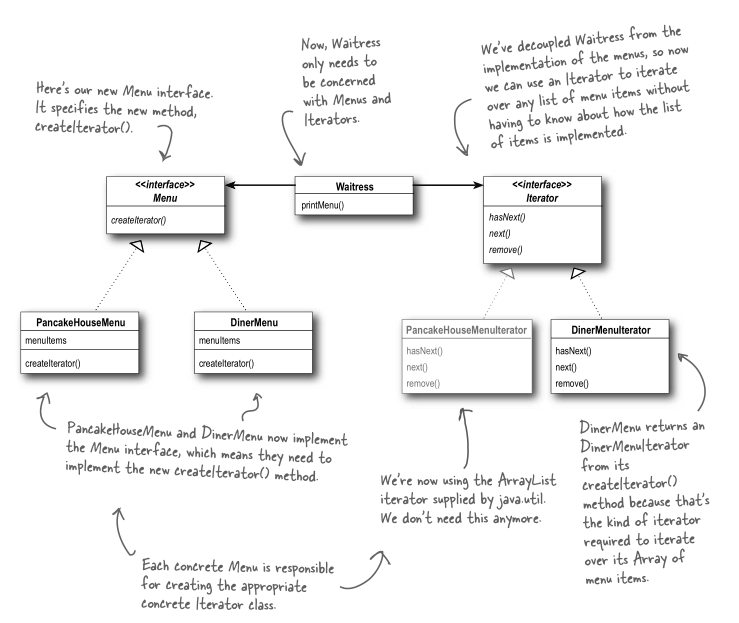
\includegraphics[width=.9\linewidth]{iterator/img/iteratorUML}
	\caption{UML-Darstellung Composite-Musters}
	\label{fig:iteratorUML}
\end{figure}


